\documentclass{article}

\usepackage[top=2.54cm, left=2.54cm, right=2.54cm, bottom=2.54cm]{geometry}
\usepackage{amsmath}
\usepackage{booktabs}
\usepackage{hyperref}
\usepackage{multicol}
\hypersetup{colorlinks=true, urlcolor=blue,}
\usepackage[svgnames]{xcolor}
\usepackage{graphicx}
\usepackage{cancel}
\usepackage{float}

\begin{document}
\noindent
Jake Mathews \hfill July 26th, 2018

\hrule
\begin{center}
\large {Homework Assignment 9}\\ \large{Simple Harmonic Motion}
\end{center}
\hrule
\vspace{1pt}
\hrule height 1pt

\section{Introduction}
The goal of this assignment is to compare the approximation of a second-order ordinary differential expression (ODE) via Euler's method to the exact numerical solution and do test whether or not total energy is conserved in the system by Euler's method. A single axis spring mass system neglecting friction, air resistance, and gravity creates a second-order ODE where energy should be conserved.\\

\noindent
Simple harmonic motion can be derived from Newton’s 2nd law:

\begin{equation}
\label{eq:1}
F = \frac{m}{a}
\end{equation}
For our case, we will assume a mass attached to a spring (horizontally) with a spring constant k. Hook’s law for this system is simply

\begin{equation}
\label{eq:2}
F = -kx
\end{equation}
where x is the displacement. Equating Eq. (\ref{eq:2}) to Eq. (\ref{eq:1}), we will obtain

\begin{equation}
\label{eq:3}
m \frac{d^2 x}{dt^2}= -kx(t)
\end{equation}
The general solution to Eq. (\ref{eq:3}) is written as

\begin{equation}
\label{eq:4}
x(t) = A \ cos(\omega t) + B \ sin(\omega t)
\end{equation}
where $\omega = \sqrt{k / m}$ and the constant coefficients A and B are obtained from the Initial Conditions (I.C.)

\begin{equation}
\label{eq:5}
x(t = 0) = x_0
	\quad\text{and}\quad  
v(t = 0) = v_0
\end{equation}
Using the I.C.’s and after some simple algebra, the position of the mass on this spring system is then

\begin{equation}
\label{eq:6}
x(t) = x_0 \ cos(\omega t) + \frac{v_0}{\sqrt{k / m}} sin(\omega t)
\end{equation}
In order to approximate the solution to Eq. (\ref{eq:3}), we first need to reduce our 2nd order ODE to two 1st order
differential equations. Following from lecture, we will have

\begin{equation}
\label{eq:7}
\frac{dx(t)}{dt} = v(t) 
	\quad\text{and}\quad  
m \frac{dv(t)}{dt} = -kx(t)
\end{equation}
Note the expressions are coupled together. By using the initial conditions in Eq. (\ref{eq:5}) we can solve the coupled ODE's

\begin{equation}
\label{eq:8}
t_1 = t_0 + \Delta t
\end{equation}
\begin{equation}
\label{eq:9}
x_1 = x_0 + v_0 \ \Delta t
\end{equation}
\begin{equation}
\label{eq:10}
v_1 = v_0 + \frac{-k \ x}{m} \Delta t
\end{equation}



\pagebreak
\section{Simulation Results}
Fig.(\ref{fig:1}) is a plot of the x position of a spring mass system at a given time ($x(t)$) versus time $(t)$. The plot shows the both the positioning of the spring mass system using an exact numerical solution with Euler's approximation overlayed to show the error.

\begin{figure}[H]
\begin{center}
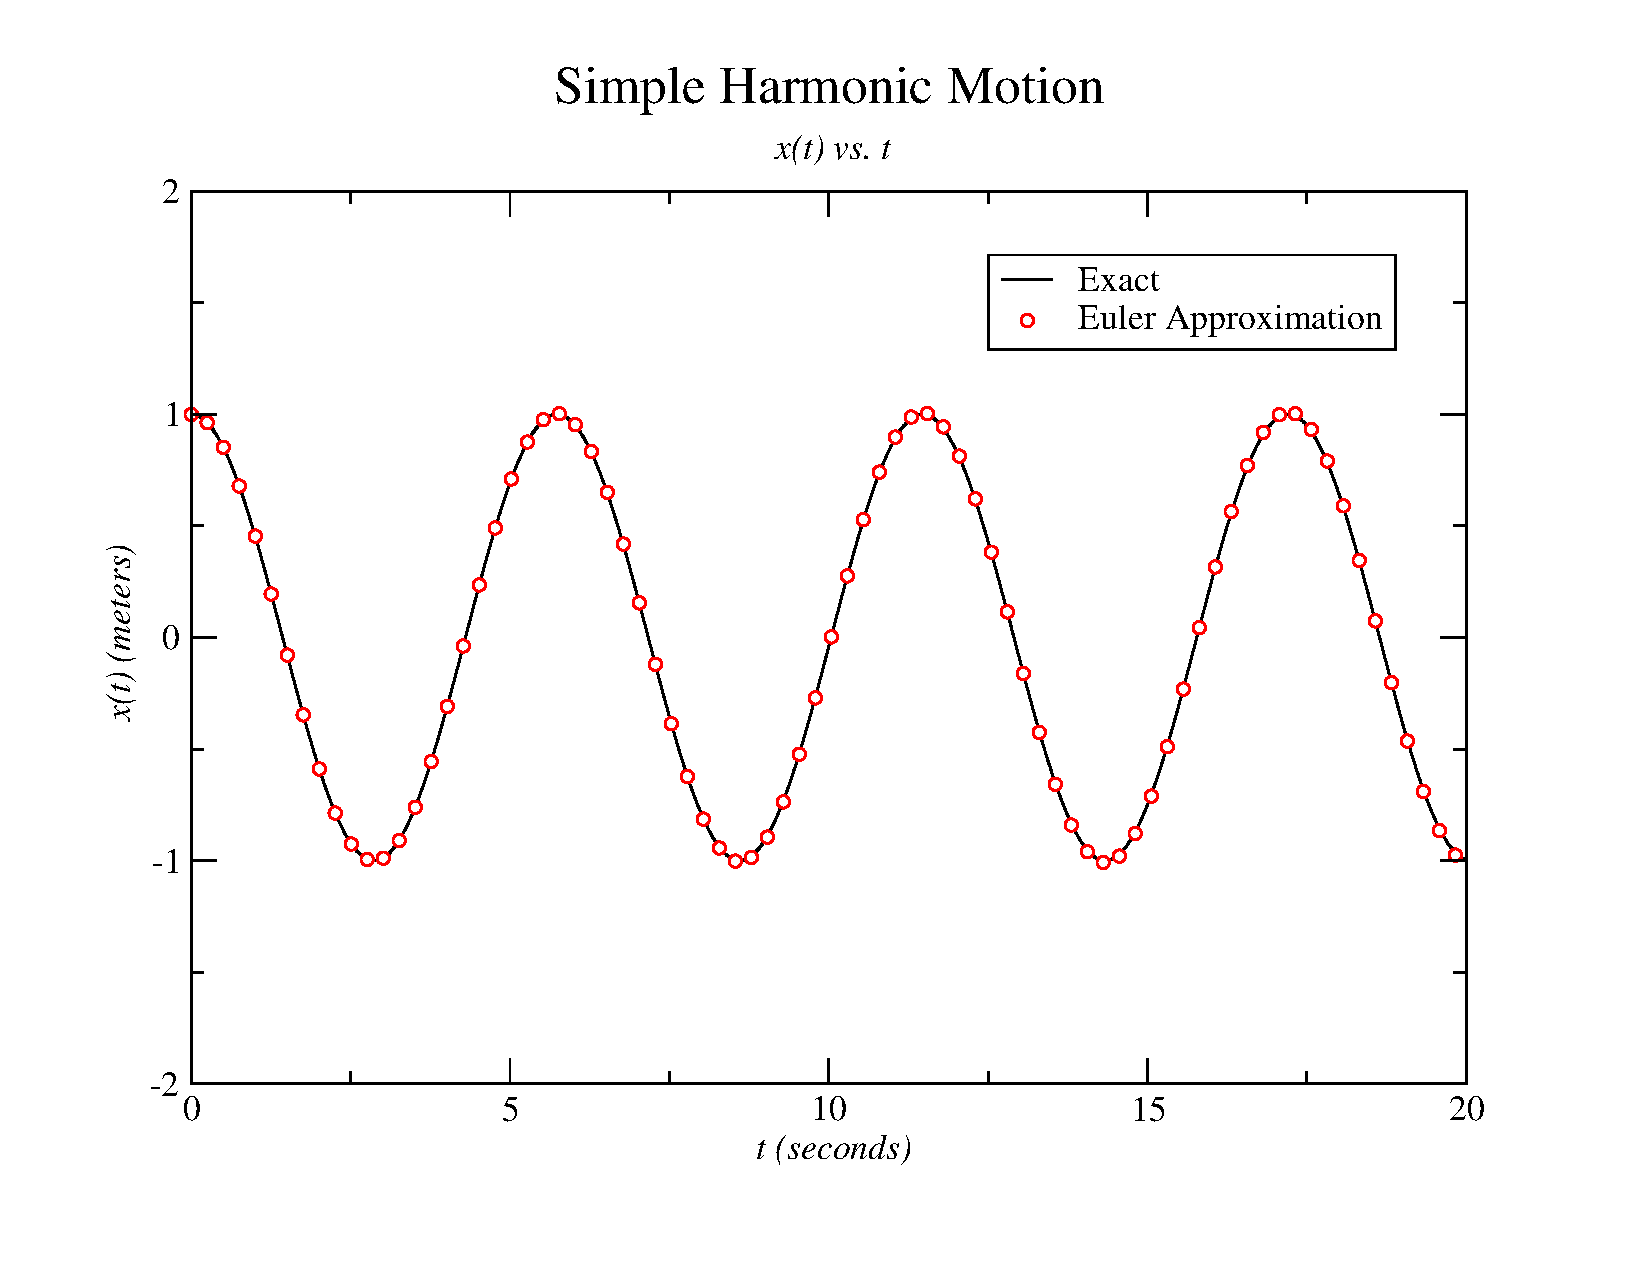
\includegraphics[scale=0.59]{./results}
\end{center}
\caption{Simple Harmonic Motion Plot}
\label{fig:1}
\end{figure} 
\noindent 
The simulation was executed with the initial conditions defined in Eq. (\ref{eq:5}) for a time of 20 seconds with a time step of 0.001 seconds which creates 20,000 data points. Based on the overlay of Euler's approximation over the exact solution in Fig. (\ref{fig:1}), it would appear as though there is little to no error on this timescale indicating that Euler's method is suitable for simulating simple systems where energy is conserved.

\pagebreak
\noindent
A way to confirm whether or not energy is concerned without manually parsing the data would be to graph the total system energy over time as seen in Fig. (\ref{fig:2}). Total energy ($E_T$) in a spring mass system such as this is the sum of the kinetic energy of the mass ($K_E$) and the potential energy of the spring ($U_E$). The kinetic energy of the mass at a given time $t$ is ,

\begin{equation}
\label{eq:12}
K_E(t) = \frac{1}{2} \ m \ v(t)^2
\end{equation}
The potential energy of the spring at a given time $t$ is,

\begin{equation}
\label{eq:13}
U_E(t) = \frac{1}{2} \ k \ x(t)^2
\end{equation}
So the total energy in the system at a given time $t$ is defined as,

\begin{equation}
\label{eq:13}
E_T(t) = \frac{1}{2} \ m \ v(t)^2 + 
			\frac{1}{2} \ k \ x(t)^2 =
			Constant
\end{equation}
Fig.(\ref{fig:2}) is a graph of the the total energy ($E_T$) of the spring mass system over time during the same 20 second simulation.

\begin{figure}[H]
\begin{center}
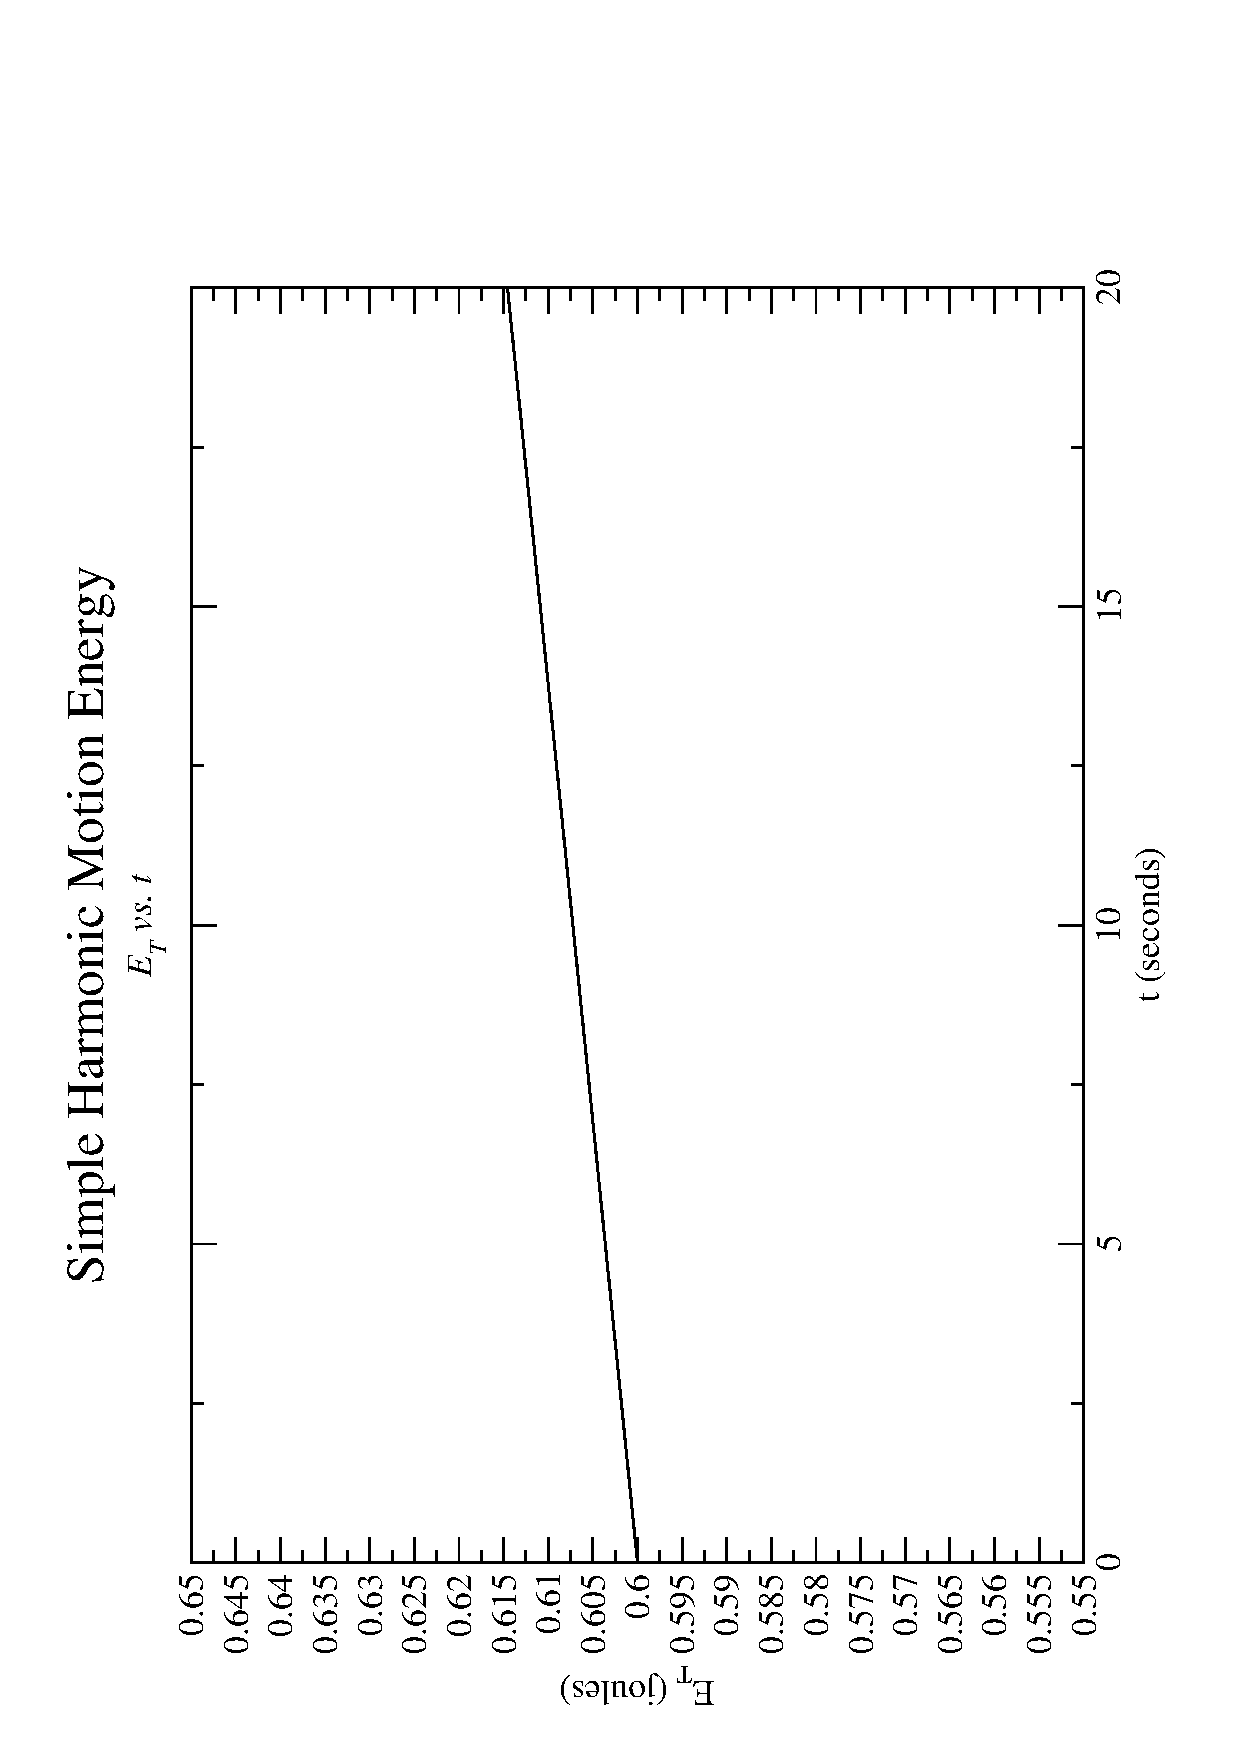
\includegraphics[scale=0.59]{./conservation}
\end{center}
\caption{Simple Harmonic Motion Energy}
\label{fig:2}
\end{figure} 

\noindent
Clearly the energy in the system is not conserved when simulating with Euler's method. The growth in energy over time is not easily detectable in the position of the spring mass system over the time scale of 20 seconds. Over the course of the simulation it would appear that the energy increasing linearly over time. To test this I ran the simulation again with a timescale of 2000 seconds. The results of which are Fig.(\ref{fig:3}) and Fig.(\ref{fig:4}).

\begin{figure}[H]
\begin{center}
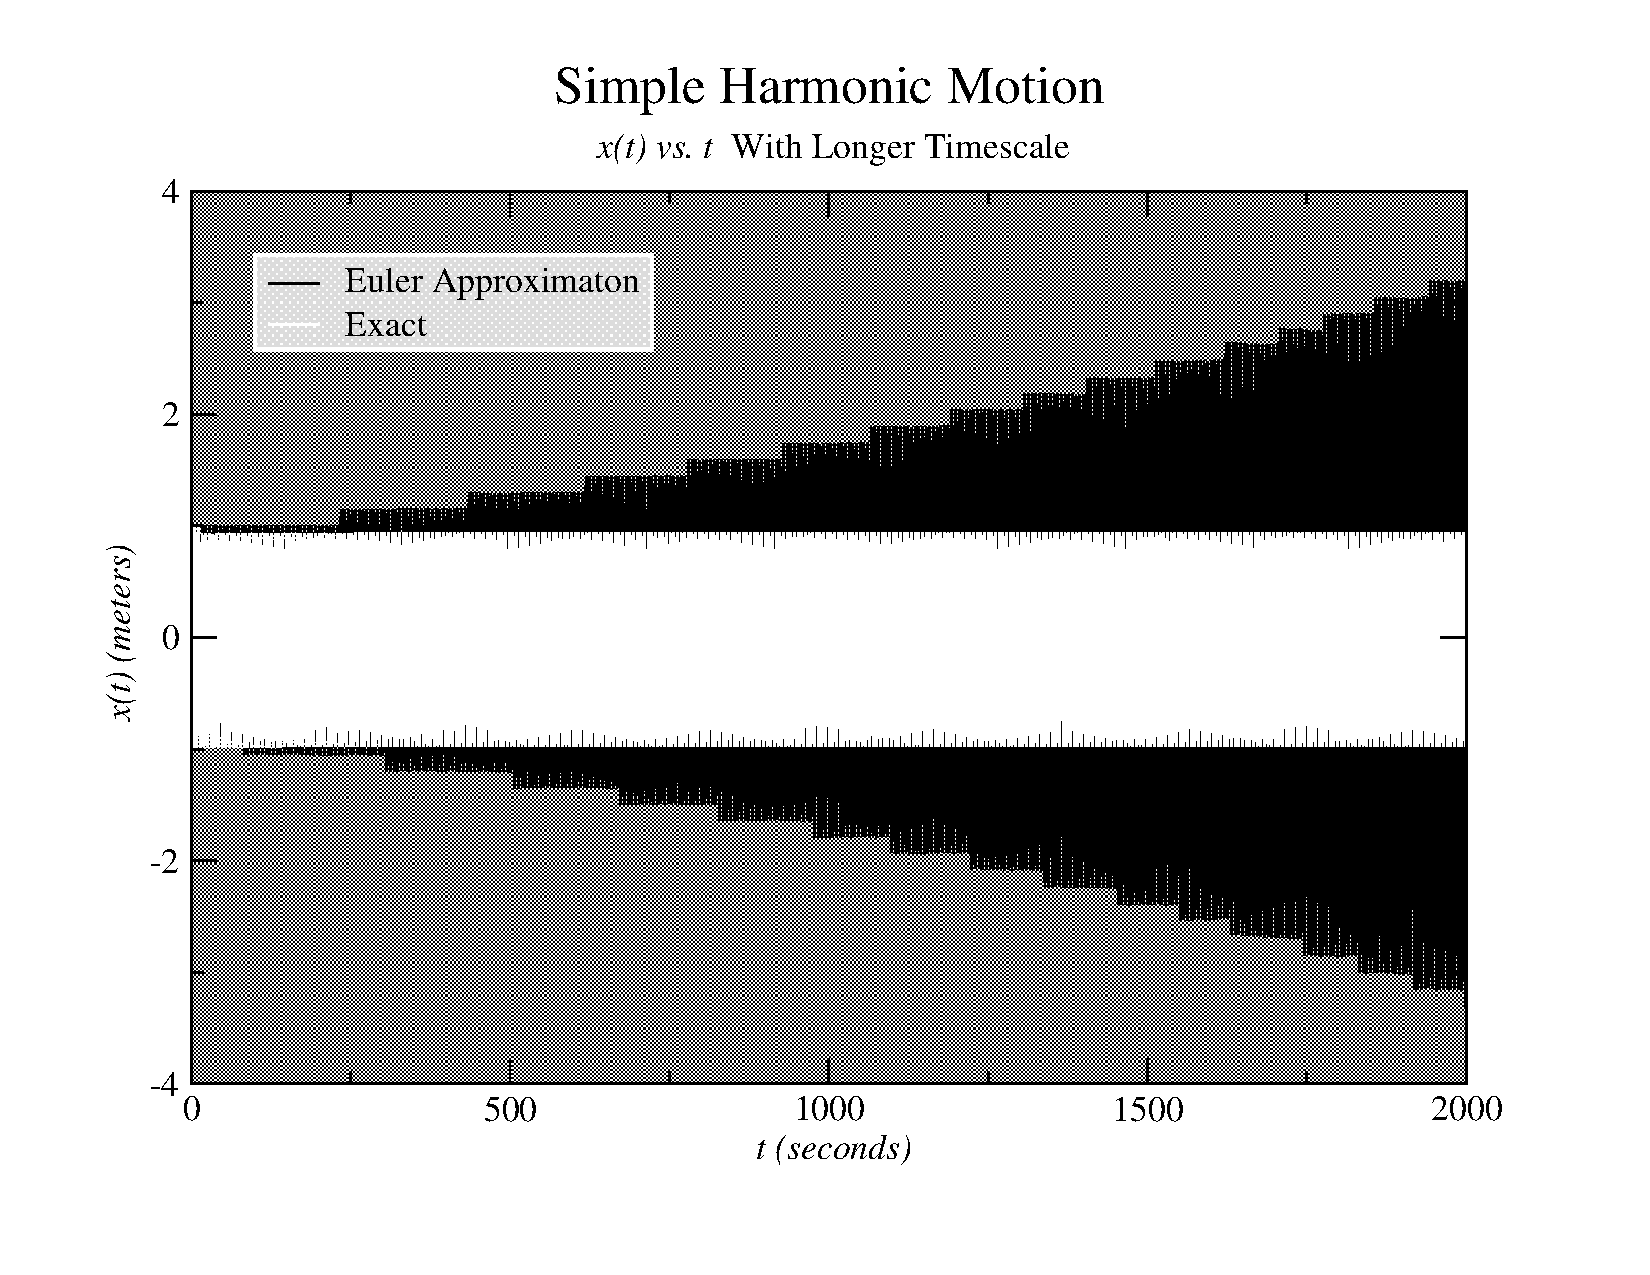
\includegraphics[scale=0.59]{./results2000}
\end{center}
\caption{Simple Harmonic Motion With Extended Timescale}
\label{fig:3}
\end{figure} 

\noindent
In Fig.(\ref{fig:3}) the approximation via Euler's method is colored black and the exact solution is colored white. Due to the amount of data points on this graph, both lines appear to be solid chunks.\\

\noindent
The exact solution continues to oscillate between 1.0 meter and -1.0 meter even on large timescales. The the error in the approximation via Euler's method differs noticeably after roughly 70 seconds and continues to accelerate as time goes on.


\begin{figure}[H]
\begin{center}
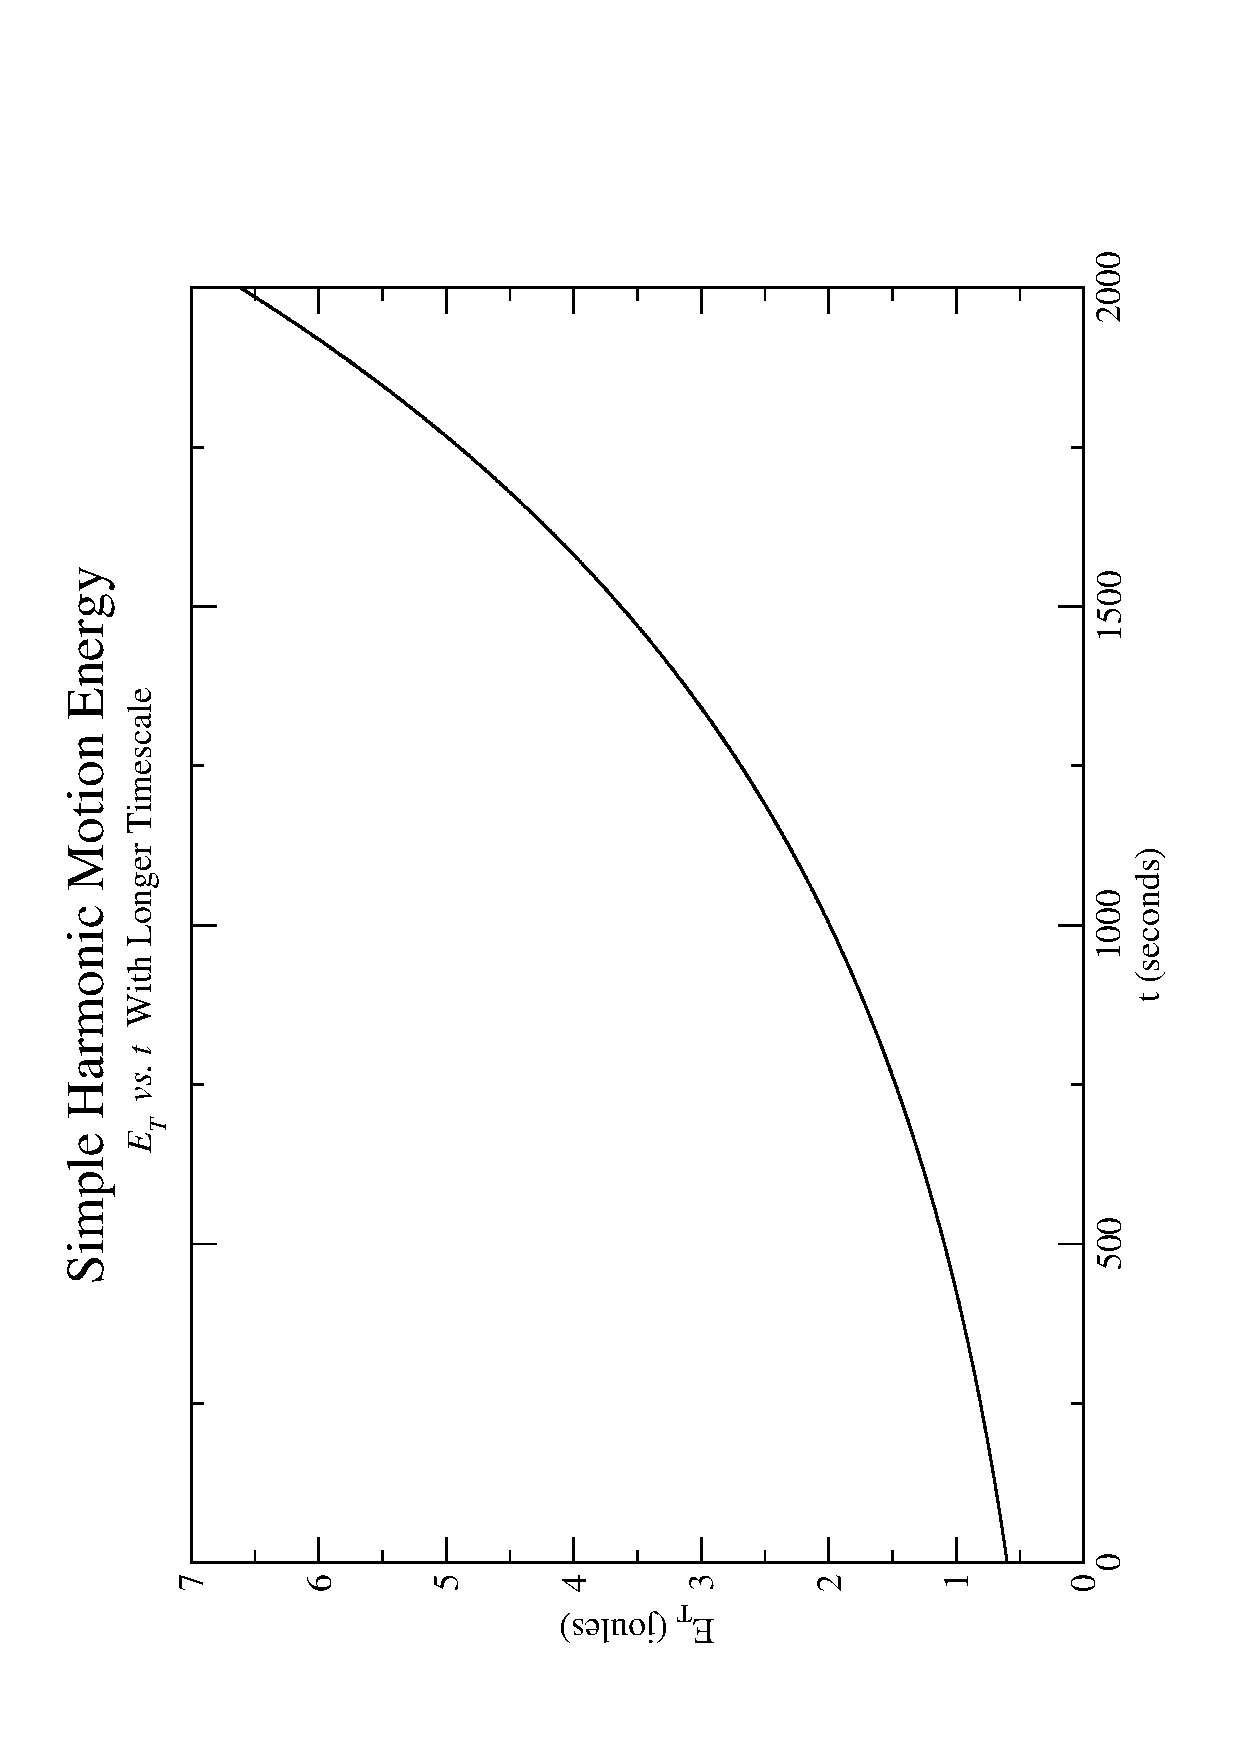
\includegraphics[scale=0.59]{./conservation2000}
\end{center}
\caption{Simple Harmonic Motion Energy With Extended Timescale}
\label{fig:4}
\end{figure} 

\noindent
In Fig. (\ref{fig:4}) the energy of the spring mass system no longer appears to be growing linearly as it did in Fig.(\ref{fig:2}), but rather growing exponentially over time.

\pagebreak
\section{The Code}
These simulation results are the product of a FORTRAN 90 program.The program will simulate the position and energy of a spring mass system in a simple harmonic motion  over time. The position in the x-axis of the spring mass system at a given time $x(t)$ and the time $t$ is written to a data file named 'exact.dat' for the exact solution and 'approximation.dat' for the approximation made with Euler's method. The position in the total energy of the spring mass system $E_T$ and the time $t$ during the approximation made with Euler's method is written to a data file named 'energy.dat'. The .dat files can be used to run statistical analysis on and/or plot the results to a graph.\\

\noindent
The exact solution is calculated by running Eq.(\ref{eq:6}) in a loop 20,000 times to simulate running for 20 seconds with a time step of 0.001 seconds. This approximated solution is calculated by running Eqs.(\ref{eq:8}, \ref{eq:9}, and \ref{eq:10}) in a loop where $\Delta t = 0.001$ seconds until $t_1$ equals or exceeds 20 seconds. $t_0$, $x_0$, and $v_0$ in Eqs.(\ref{eq:8}, \ref{eq:9}, and \ref{eq:10}) are replaced with the previous iterations results starting with the initial conditions outlined in Eq.(\ref{eq:5})

\section{Conclusion}
Figures (\ref{fig:2}, \ref{fig:3}, and \ref{fig:4}) show that energy is not conserved when approximating the position of continuous systems, such as orbits and SHO's, using Euler's method. The total energy of the system has an error in the approximation. Since Euler's method iterates based on the previous calculations results, the error increases exponentially over time as seen in Fig.(\ref{fig:4}).\\

\noindent
A popular alternative to Euler's method is to pick one of the variations of the Runge-Kutta method such as Runge-Kutta 2 (RK2) or Runge-Kutta 4 (RK4).

\end{document}
